\documentclass[paper=a4, fontsize=11pt]{scrartcl} % A4 paper and 11pt font size

\usepackage[T1]{fontenc} % Use 8-bit encoding that has 256 glyphs
\usepackage{fourier} % Use the Adobe Utopia font for the document - comment this line to return to the LaTeX default
\usepackage[english]{babel} % English language/hyphenation
\usepackage{amsmath,amsfonts,amsthm} % Math packages
\usepackage{graphicx}
\graphicspath{ {./images/} }
\usepackage{lipsum} % Used for inserting dummy 'Lorem ipsum' text into the template

\usepackage{sectsty} % Allows customizing section commands
\allsectionsfont{\centering \normalfont\scshape} % Make all sections centered, the default font and small caps

\usepackage{fancyhdr} % Custom headers and footers
\pagestyle{fancyplain} % Makes all pages in the document conform to the custom headers and footers
\fancyhead{} % No page header - if you want one, create it in the same way as the footers below
\fancyfoot[L]{} % Empty left footer
\fancyfoot[C]{} % Empty center footer
\fancyfoot[R]{\thepage} % Page numbering for right footer
\renewcommand{\headrulewidth}{0pt} % Remove header underlines
\renewcommand{\footrulewidth}{0pt} % Remove footer underlines
\setlength{\headheight}{13.6pt} % Customize the height of the header

\numberwithin{equation}{section} % Number equations within sections (i.e. 1.1, 1.2, 2.1, 2.2 instead of 1, 2, 3, 4)
\numberwithin{figure}{section} % Number figures within sections (i.e. 1.1, 1.2, 2.1, 2.2 instead of 1, 2, 3, 4)
\numberwithin{table}{section} % Number tables within sections (i.e. 1.1, 1.2, 2.1, 2.2 instead of 1, 2, 3, 4)

\setlength\parindent{0pt} % Removes all indentation from paragraphs - comment this line for an assignment with lots of text

%----------------------------------------------------------------------------------------
%	TITLE SECTION
%----------------------------------------------------------------------------------------

\newcommand{\horrule}[1]{\rule{\linewidth}{#1}} % Create horizontal rule command with 1 argument of height
\newcommand{\itab}[1]{\hspace{0em}\rlap{#1}}
\newcommand{\tab}[1]{\hspace{.2\textwidth}\rlap{#1}}

\title{	
\normalfont \normalsize 
\textsc{University of Maryland, Baltimore County} \\ [25pt] % Your university, school and/or department name(s)
\horrule{0.5pt} \\[0.4cm] % Thin top horizontal rule
\huge CMSC678 Homework 1  \\ % The assignment title
\horrule{2pt} \\[0.5cm] % Thick bottom horizontal rule
}

\author{Yin Huang} % Your name

\date{\normalsize\today} % Today's date or a custom date

\begin{document}

\maketitle % Print the title

%----------------------------------------------------------------------------------------
%	PROBLEM 1
%----------------------------------------------------------------------------------------

\section{Problem One}
In this part of the assignment you will gain familiarity with WEKA, the Waikato Environment for Knowledge Analysis. WEKA is widely used in the machine learning and data mining communities because, among other things, it provides both a nice user interface to a number of standard algorithms and a Java API.

First, you must download WEKA from the following URL: http://www.cs.waikato.ac.nz/ml/weka/. 

The "Getting Started" section of that page has links for information on system requirements, how to download the software, and documentation. WEKA is written in Java and should run on any platform with Java 1.5 or higher.

Read about the Adult Census Income dataset, and get it in the form of an ARFF file. Then do the following: 

\begin{itemize}
 \item  Build a decision tree (J48 classifier) with the default parameters and report the (stratified cross-validation) accuracy.
  \item  Now turn off pruning and report the accuracy. Inspect the output of the algorithm. Has it overfit? How can you tell?
  \item  Build a decision stump (a decision tree with a single split; you can find it in the tree section of algorithms in Weka) and report the accuracy. Inspect the output of the algorithm. Has it underfit? How can you tell?

\end{itemize}
%------------------------------------------------
\paragraph{Answer 1}
Below is the screen-shot of J48 classifier with the default parameters: \\
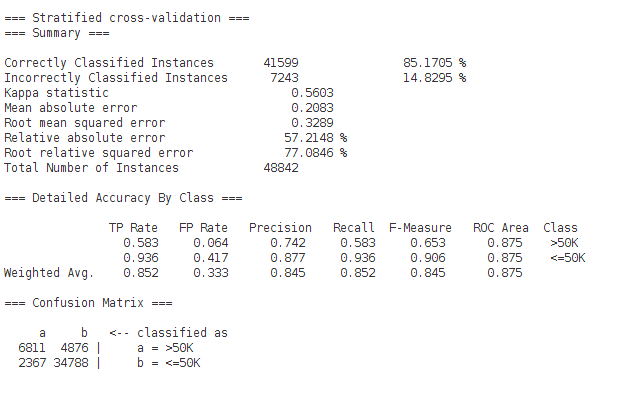
\includegraphics[scale=0.65]{question1.png}\label{Summary for default parameters J48 classifier} \\
Number of Leaves  : 	689   Size of the tree : 	834 
\paragraph{Answer 2}
Below is the screen-shot of J48 classifier without pruning: \\
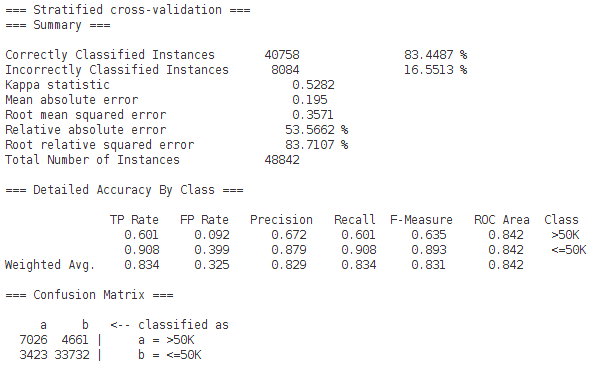
\includegraphics[scale=0.65]{question2.png}\label{Summary for default parameters J48 classifier without prunning} \\
Number of Leaves  : 	13074  Size of the tree : 	14871
Given the fact that the total size of the training set is 48842, and the output size of our decision tree is 14871 with 13074 leaves, we can safely assume this is overfitting because almost one quoter of our training set is used to build the decision tree. In a word, our tree has a high variance but low bias. In order to verify our assumption, we need to test the accuracy using other test data with no overlapping datasets with our training set.

\paragraph{Answer 3}
Below is the screen-shot of a decision dump with our dataset. 
\begin{center}
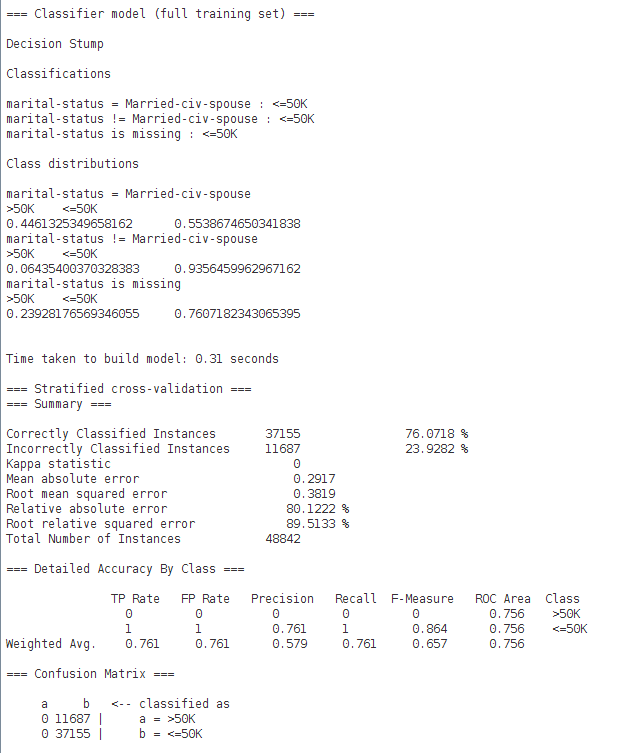
\includegraphics[scale=0.6]{question3.png}\label{Summary for a decision dump tree} \\
\end{center}
As we can see, the tree is only testing on one feature: marital-status and then give us the income label. This is absolutely underfitting since we have 15 attributes. In a word, our tree has a high bias but low variance. 

%----------------------------------------------------------------------------------------
%	PROBLEM 2
%----------------------------------------------------------------------------------------

\section{Problem Two}

%------------------------------------------------
In this part of the homework you will implement k-means clustering and experiment with different ways of initializing the cluster centroids.

The MNIST dataset is a well-studied collection of handwritten digits. It is often used to test multi-class classification algorithms, where there is one class for each of the 10 digits (0 - 9). In this homework, you will use it for unsupervised clustering.

I've made two files available for you: 
\begin{itemize}


  \item  The raw MNIST data, which is a text file containing 10,000 rows. Each row contains 28 * 28 = 784 integers in the range 0 to 255. Each integer is the pixel value from a 28 x 28 image of a handwritten digit. Every row corresponds to a vector in the dataset that is to be clustered.
  \item  The labels for the raw data are in a file with 10,000 rows. The first row contains the correct digit label for the first row in the raw data. The second row is the label for the second instance, and so on. 

\end{itemize}

 Implement the k-means clustering algorithm. You will only use your algorithm for this dataset, so you can hard-wire in the number of instances and the size of each instance.\\
 The goal is not to write a generic version of the algorithm (though you can if you wish). The goal is to understand how it works on real data. You will need to try different values of k so that must be a parameter.

After completing the implementation (and testing for correctness, of course), do the following: 
\begin{itemize}

 \item  Randomly sample k = 10 instances, use them as the initial cluster centroids, and run the algorithm to covergence. For each cluster, find the most common digit in that cluster and count the number of instances in the cluster that are different from the most common one. Sum that count over all of the clusters.
 \item   Repeat the above step 10 times in total and report the average number of iterations to convergence and the average number of instances that are in the wrong cluster.
 \item   Run the algorithm with k = 5. Look at the clusters and see if there are digits that tend to get grouped together. What are they and explain why you think they are grouped into the same cluster.
  \item  Finally, run the algorithm 10 times again with k = 10 and report the same information as above (iterations to convergence and number of wrongly clustered instances). But this time do not choose random instances for the cluster centroids. Randomly choose an instance that represents each of the digits and use them as the centroids. That is, one of the centroids will be a randomly chose 0, another will be a randomly chose 1, and so on. Do you observe any difference in the performance statistics? Why or why not?
 \item   Turn in hard copy of your code. 

\end{itemize}
%----------------------------------------------------------------------------------------

\end{document}
